\newif\ifshowsolutions
\showsolutionstrue
\documentclass{article}
\usepackage{listings}
\usepackage{amsmath}
\usepackage{subfig}
\usepackage{amsthm}
\usepackage{amsmath}
\usepackage{amssymb}
\usepackage{graphicx}
\usepackage{mdwlist}
\usepackage{geometry}
\usepackage{titlesec}
\usepackage{palatino}
\usepackage{mathrsfs}
\usepackage{fancyhdr}
\usepackage{paralist}
\usepackage{todonotes}
\usepackage{tikz}
\usepackage{float} % Place figures where you ACTUALLY want it
\usepackage{comment} % A hack to toggle sections
\usepackage{ifthen}
\usepackage{mdframed}
\usepackage{verbatim}
\usepackage{listings}
\usepackage{bbm}
\usepackage{upquote} % Prevents backticks replacing single-quotes in verbatim
\usepackage[strings]{underscore}
\usepackage[colorlinks=true]{hyperref}
\usetikzlibrary{positioning,shapes,backgrounds}

\geometry{margin=1in}
\geometry{headheight=2in}
\geometry{top=2in}

\setlength{\marginparwidth}{2.15cm}
\setlength{\parindent}{0em}
\setlength{\parskip}{0.6\baselineskip}

\rhead{}
\lhead{}

% Spacing settings.
\titlespacing\section{0pt}{12pt plus 2pt minus 2pt}{0pt plus 2pt minus 2pt}
\titlespacing\subsection{0pt}{12pt plus 4pt minus 2pt}{0pt plus 2pt minus 2pt}
\titlespacing\subsubsection{0pt}{12pt plus 4pt minus 2pt}{0pt plus 2pt minus 2pt}
\renewcommand{\baselinestretch}{1.15}

% Shortcuts for commonly used operators.
\newcommand{\E}{\mathbb{E}}
\newcommand{\Var}{\operatorname{Var}}
\newcommand{\Cov}{\operatorname{Cov}}
\newcommand{\Bias}{\operatorname{Bias}}
\DeclareMathOperator{\argmin}{arg\,min}
\DeclareMathOperator{\argmax}{arg\,max}

% Do not number subsections and below.
\setcounter{secnumdepth}{1}

% Custom format subsection.
\titleformat*{\subsection}{\large\bfseries}

% Set up the problem environment.
\newcounter{problem}[section]
\newenvironment{problem}[1][]
  {\begingroup
    \setlength{\parskip}{0em}
    \refstepcounter{problem}\par\addvspace{1em}\textbf{Problem~\Alph{problem}\!
    \ifthenelse{\equal{#1}{}}{}{ [#1 points]}:}
  \endgroup}

% Set up the subproblem environment.
\newcounter{subproblem}[problem]
\newenvironment{subproblem}[1][]
  {\begingroup
    \setlength{\parskip}{0em}
    \refstepcounter{subproblem}\par\medskip\textbf{\roman{subproblem}.\!
    \ifthenelse{\equal{#1}{}}{}{ [#1 points]:}}
  \endgroup}

% Set up the teachers and materials commands.
\newcommand\teachers[1]
  {\begingroup
    \setlength{\parskip}{0em}
    \vspace{0.3em} \textit{\hspace*{2em} TAs responsible: #1} \par
  \endgroup}
\newcommand\materials[1]
  {\begingroup
    \setlength{\parskip}{0em}
    \textit{\hspace*{2em} Relevant materials: #1} \par \vspace{1em}
  \endgroup}

% Set up the hint environment.
\newenvironment{hint}[1][]
  {\begin{em}\textbf{Hint: }}
  {\end{em}}


% Set up the solution environment.
\ifshowsolutions
  \newenvironment{solution}[1][]
    {\par\medskip \begin{mdframed}\textbf{Solution~\Alph{problem}#1:} \begin{em}}
    {\end{em}\medskip\end{mdframed}\medskip}
  \newenvironment{subsolution}[1][]
    {\par\medskip \begin{mdframed}\textbf{Solution~\Alph{problem}#1.\roman{subproblem}:} \begin{em}}
    {\end{em}\medskip\end{mdframed}\medskip}
\else
  \excludecomment{solution}
  \excludecomment{subsolution}
\fi


%%%%%%%%%%%%%%%%%%%%%%%%%%%%%%
% HEADER
%%%%%%%%%%%%%%%%%%%%%%%%%%%%%%

\chead{
  {\vbox{
      \vspace{2mm}
      \large
      Machine Learning \& Data Mining \hfill
      Caltech CS/CNS/EE 155 \hfill \\[1pt]
      Set 1\hfill
      January $8^{th}$, 2019 \\
    }
  }
}

\begin{document}
\pagestyle{fancy}



%%%%%%%%%%%%%%%%%%%%%%%%%%%%%%
% POLICIES
%%%%%%%%%%%%%%%%%%%%%%%%%%%%%%

\section*{Policies}
\begin{itemize}
  \item Due 9 PM, January $16^\text{th}$. 
  \item Note: both the moodle submission AND Gradescope submissions must be submitted by the deadline
  \item You are free to collaborate on all of the problems, subject to the collaboration policy stated in the syllabus.
  \item If you have trouble with this homework, it may be an indication that you should drop the class.
  \item You should submit all code used in the homework. We ask that you use Python 3 and sklearn version $\geq$0.18 for your code, and that you comment your code such that the TAs can follow along and run it without any issues. 
\end{itemize}

\section*{Submission Instructions}
\textbf{PLEASE NOTE} that there are two steps to submitting your Problem Set. Both must be submitted by the deadline. For the course's late submission policy, please refer to the course website.

\begin{itemize}
   \item Please submit your report as a single .pdf file to Gradescope (entry code 9EJKYV), under "Set 1 Report". \textbf{In the report, include any images generated by your code along with your answers to the questions.} For instructions specifically pertaining to the Gradescope submission process, see \url{https://www.gradescope.com/get_started#student-submission}.
   \item Please submit your code as a .zip archive to Moodle, with filename \texttt{LastnameFirstname.zip} (replacing \texttt{Lastname} with your last name and \texttt{Firstname} with your first name). The .zip file should contain your code files. Submit your code either as Jupyter notebook .ipynb files or .py files. 
\end{itemize}

%%%%%%%%%%%%%%%%%%%%%%%%%%%%%%
% PROBLEM 1
%%%%%%%%%%%%%%%%%%%%%%%%%%%%%%

\newpage
\section{Basics [16 Points]}
\materials{lecture 1}

Answer each of the following problems with 1-2 short sentences.

\begin{problem}[2]
  What is a hypothesis set?
\end{problem}
\begin{solution}
  
\end{solution}

\begin{problem}[2]
  What is the hypothesis set of a linear model?
\end{problem}
\begin{solution}
  
\end{solution}

\begin{problem}[2]
  What is overfitting?
\end{problem}
\begin{solution}
  
\end{solution}

\begin{problem}[2]
  What are two ways to prevent overfitting?
\end{problem}
\begin{solution}
  
\end{solution}

\begin{problem}[2]
  What are training data and test data, and how are they used differently? Why should you never change your model based on information from test data?
\end{problem}
\begin{solution}
  
\end{solution}

\begin{problem}[2]
  What are the two assumptions we make about how our dataset is sampled?
\end{problem}
\begin{solution}
  
\end{solution}

\begin{problem}[2]
  Consider the machine learning problem of deciding whether or not an email is spam. What could $X$, the input space, be? What could $Y$, the output space, be?
\end{problem}
\begin{solution}
  
\end{solution}

\begin{problem}[2]
  What is the $k$-fold cross-validation procedure?
\end{problem}
\begin{solution}
  
\end{solution}



%%%%%%%%%%%%%%%%%%%%%%%%%%%%%%
% PROBLEM 2
%%%%%%%%%%%%%%%%%%%%%%%%%%%%%%

\newpage
\section{Bias-Variance Tradeoff [34 Points]}
\materials{lecture 1}

\begin{problem}[5]
  Derive the bias-variance decomposition for the squared error loss function. That is, show that for a model $f_S$ trained on a dataset $S$ to predict a target $y(x)$ for each $x$,
  \begin{align*}
    \E_S \left[E_\text{out}\left(f_S\right)\right] = \E_x[\Bias(x) + \Var(x)]
  \end{align*}
  given the following definitions:
  \begin{align*}
    F(x) &= \E_S\left[f_S(x) \right] \\
    E_\text{out}(f_S) &= \E_x\left[\left(f_S(x) - y(x)\right)^2\right] \\
    \Bias(x) &= (F(x) - y(x))^2 \\
    \Var(x) &= \E_S\left[(f_S(x)-F(x))^2\right]
  \end{align*}
\end{problem}

\begin{solution}
  
\end{solution}

In the following problems you will explore the bias-variance tradeoff by producing learning curves for polynomial regression models.

A \emph{learning curve} for a model is a plot showing both the training error and the cross-validation error as a function of the number of points in the training set. These plots provide valuable information regarding the bias and variance of a model and can help determine whether a model is over-- or under--fitting.

\emph{Polynomial regression} is a type of regression that models the target $y$ as a degree--$d$ polynomial function of the input $x$. (The modeler chooses $d$.)  You don't need to know how it works for this problem, just know that it produces a polynomial that attempts to fit the data.

\begin{problem}[14]
    Use the provided \texttt{2_notebook.ipynb} Jupyter notebook to enter your code for this question. This notebook contains examples of using NumPy's polyfit and polyval methods, and scikit-learn's KFold method; you may find it helpful to read through and run this example code prior to continuing with this problem. Additionally, you may find it helpful to look at the documentation for scikit-learn's learning_curve method for some guidance.

The dataset \texttt{bv_data.csv} is provided and has a header denoting which columns correspond to which values. Using this dataset, plot learning curves for 1st--, 2nd--, 6th--, and 12th--degree polynomial regression (4 separate plots) by following these steps for each degree $d \in \{1, 2, 6, 12\}$:

\newpage

  \begin{enumerate}
    \item For each $N \in \{20, 25, 30, 35, \cdots, 100\}$:
    \begin{enumerate}[i.]
      \item Perform 5-fold cross-validation on the first $N$ points in the dataset (setting aside the other points), computing the both the training and validation error for each fold. 
      \begin{itemize}
        \item Use the mean squared error loss as the error function.
        \item Use NumPy's polyfit method to perform the degree--$d$ polynomial regression and NumPy's polyval method to help compute the errors.  (See the example code and \href{https://docs.scipy.org/doc/NumPy/reference/routines.polynomials.poly1d.html}{NumPy documentation} for details.)
        \item When partitioning your data into folds, although in practice you should randomize your partitions, for the purposes of this set, simply divide the data into $K$ contiguous blocks.
      \end{itemize}
      \item Compute the average of the training and validation errors from the 5 folds.
    \end{enumerate}
    \item Create a learning curve by plotting both the average training and validation error as functions of $N$.
  \end{enumerate}

\end{problem}
\begin{solution}
  \end{solution}

\begin{problem}[3]
  Based on the learning curves, which polynomial regression model (i.e. which degree polynomial) has the highest bias? How can you tell?
\end{problem}
\begin{solution}

\end{solution}

\begin{problem}[3]
  Which model has the highest variance? How can you tell?
\end{problem}
\begin{solution}
  
\end{solution}

\begin{problem}[3]
  What does the learning curve of the quadratic model tell you about how much the model will improve if we had additional training points?
\end{problem}
\begin{solution}

\end{solution}

\begin{problem}[3]
  Why is training error generally lower than validation error?
\end{problem}
\begin{solution}
  
\end{solution}

\begin{problem}[3]
  Based on the learning curves, which model would you expect to perform best on some unseen data drawn from the same distribution as the training data, and why?
\end{problem}
\begin{solution}
  
\end{solution}




%%%%%%%%%%%%%%%%%%%%%%%%%%%%%%
% PROBLEM 3
%%%%%%%%%%%%%%%%%%%%%%%%%%%%%%

\newpage
\section{The Perceptron [14 Points]}
\materials{lecture 2}

The perceptron is a simple linear model used for binary classification. For an input vector $\mathbf{x} \in \mathbb{R}^d$, weights $\mathbf{w} \in \mathbb{R}^d$, and bias $b \in \mathbb{R}$, a perceptron $f: \mathbb{R}^d \rightarrow \{-1,1\}$ takes the form
\begin{align*}
  f(\mathbf{x}) = \operatorname{sign}\left(\left(\sum_{i=1}^d w_i x_i\right) + b \right)
\end{align*}

The weights and bias of a perceptron can be thought of as defining a hyperplane that divides $\mathbb{R}^d$ such that each side represents an output class. For example, for a two dimensional dataset, a perceptron could be drawn as a line that separates all points of class $+1$ from all points of class $-1$.

The PLA (or the Perceptron Learning Algorithm) is a simple method of training a perceptron. First, an initial guess is made for the weight vector $\mathbf{w}$. Then, one misclassified point is chosen arbitrarily and the $\mathbf{w}$ vector is updated by
\begin{align*}
  \mathbf{w}_{t+1} &= \mathbf{w}_t + y(t)\mathbf{x}(t) \\
  b_{t + 1} &= b_t + y(t),
\end{align*}

where $\mathbf{x}(t)$ and $y(t)$ correspond to the misclassified point selected at the $t^\text{th}$ iteration.
This process continues until all points are classified correctly.

The following few problems ask you to work with the provided Jupyter notebook for this problem, titled \texttt{3_notebook.ipynb}. This notebook utilizes the file \texttt{perceptron_helper.py}, but you should not need to modify this file.

\begin{problem}[8]
  The graph below shows an example 2D dataset. The $+$ points are in the $+1$ class and the $\circ$ point is in the $-1$ class. 

  \begin{figure}[H]
    \centering
    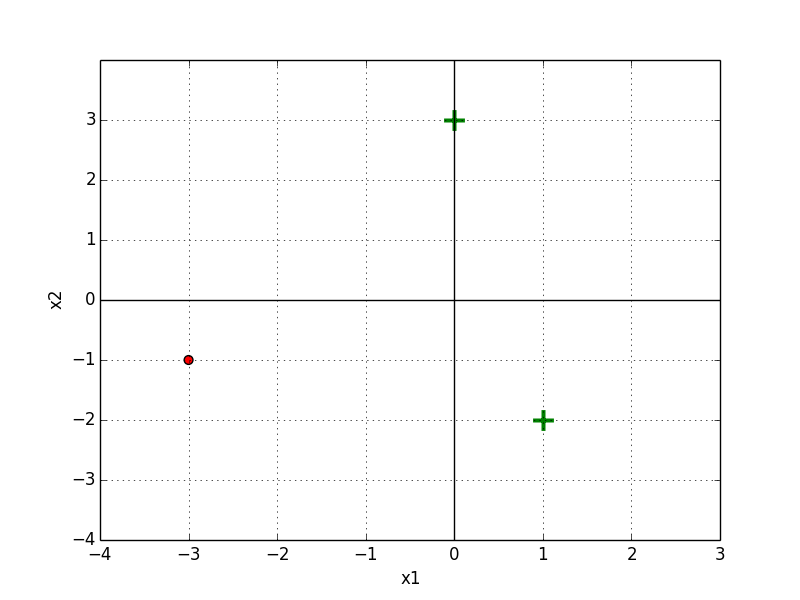
\includegraphics[width=0.4\textwidth]{images/perceptron.png}
    \caption{The green $+$ are positive and the red $\circ$ is negative}
    \label{fig:figure1}
  \end{figure}
  
 Implement the \texttt{update_perceptron} and \texttt{run_perceptron} methods in the notebook, and perform the perceptron algorithm with initial weights $w_1 = 0, w_2 = 1, b = 0$.

  Give your solution in the form a table showing the weights and bias at each timestep and the misclassified point $([x_1,x_2],y)$ that is chosen for the next iteration's update. You can iterate through the three points in any order. Your code should output the values in the table below; cross-check your answer with the table to confirm that your perceptron code is operating correctly.

  \begin{table}[H]
    \centering

    \begin{tabular}{l|lll|ll|l}
    \hline

    \hline
    $t$ & $b$ & $w_1$ & $w_2$ & $x_1$ & $x_2$ & $y$ \\
    \hline
      0  &  0 & 0 & 1  & 1 & -2 & +1\\
      1  &  1 & 1 & -1 & 0 & 3 & +1\\
      2  &  2 & 1 & 2 & 1 & -2 & +1\\
      3  &  3 & 2 & 0 \\
    \hline
    \end{tabular}
  \end{table}
  
  Include in your report both: the table that your code outputs, as well as the plots showing the perceptron's classifier at each step (see notebook for more detail).
  
  
\end{problem}
\begin{solution}


\end{solution}

\begin{problem}[4]
  A dataset $S = \{(\mathbf{x}_1, y_1),\cdots,(\mathbf{x}_N, y_N)\} \subset \mathbb{R}^d \times \mathbb{R}$ is \emph{linearly separable} if there exists a perceptron that correctly classifies all data points in the set. In other words, there exists a hyperplane that separates positive data points and negative data points.

  In a 2D dataset, how many data points are in the smallest dataset that is not linearly separable, such that no three points are collinear? How about for a 3D dataset such that no four points are coplanar? Please limit your solution to a few lines - you should justify but not prove your answer.

  Finally, how does this generalize for an $N$-dimensional set, in which \textbf{no} $<$$N$-dimensional hyperplane contains a non-linearly-separable subset? For the $N$-dimensional case, you may state your answer without proof or justification.
\end{problem}
\begin{solution}

\end{solution}

\begin{problem}[2]
  Run the visualization code in the Jupyter notebook section corresponding to question C (report your plots). Assume a dataset is \emph{not} linearly separable. Will the Perceptron Learning Algorithm ever converge? Why or why not?
\end{problem}
\begin{solution}

\end{solution}



%%%%%%%%%%%%%%%%%%%%%%%%%%%%%%
% PROBLEM 4
%%%%%%%%%%%%%%%%%%%%%%%%%%%%%%

\newpage
\section{Stochastic Gradient Descent [36 Points]}
\materials{lecture 2}

Stochastic gradient descent (SGD) is an important optimization method in machine learning, used everywhere from logistic regression to training neural networks. In this problem, you will be asked to first implement SGD for linear regression using the squared loss function. Then, you will analyze how several parameters affect the learning process.

Linear regression learns a model of the form:
\begin{align*}
  f(x_1, x_2, \cdots, x_d) = \left(\sum_{i=1}^d w_i x_i\right) + b
\end{align*}

% problem A tests the students understanding of matrix representations and serves are a reminder that the bias term is still there.
\begin{problem}[2]
  We can make our algebra and coding simpler by writing $f(x_1, x_2, \cdots, x_d) = \mathbf{w}^T\mathbf{x}$ for vectors $\mathbf{w}$ and $\mathbf{x}$.  But at first glance, this formulation seems to be missing the bias term $b$ from the equation above.  How should we define $\mathbf{x}$ and $\mathbf{w}$ such that the model includes the bias term?
\end{problem}
\begin{hint}
  Include an additional element in $\mathbf{w}$ and $\mathbf{x}$.
\end{hint}
\begin{solution}
  
\end{solution}

Linear regression learns a model by minimizing the squared loss function $L$, which is the sum across all training data $\{(\mathbf{x}_1, y_1),\cdots,(\mathbf{x}_N, y_N)\}$ of the squared difference between actual and predicted output values:
\[L(f) = \sum_{i=1}^N (y_i - \mathbf{w}^T\mathbf{x}_i)^2\]

\begin{problem}[2]
  SGD uses the gradient of the loss function to make incremental adjustments to the weight vector $\mathbf{w}$. Derive the gradient of the squared loss function with respect to $\mathbf{w}$ for linear regression.
\end{problem}
\begin{solution}
  
\end{solution}

The following few problems ask you to work with the first of two provided Jupyter notebooks for this problem, \texttt{4_notebook_part1.ipynb}, which includes tools for gradient descent visualization. This notebook utilizes the files \texttt{sgd_helper.py} and \texttt{multiopt.mp4}, but you should not need to modify either of these files. In addition, to run the animation code provided in this notebook, you may need to install ImageMagick. For step-by-step instructions on installing ImageMagick, please refer to the file \texttt{installing_ImageMagick.pdf}.

\newpage

For your implementation of problems C-E, \textbf{do not} consider the bias term.

\begin{problem}[8]
  Implement the \texttt{loss}, \texttt{gradient}, and \texttt{SGD} functions, defined in the notebook, to perform SGD, using the guidelines below:

  \begin{itemize}
    \item Use a squared loss function.
    \item Terminate the SGD process after a specified number of epochs, where each epoch performs one SGD iteration for each point in the dataset.
    \item It is recommended, but not required, that you shuffle the order of the points before each epoch such that you go through the points in a random order. You can use \texttt{numpy.random.permutation}.
    \item Measure the loss after each epoch. Your \texttt{SGD} function should output a vector with the loss after each epoch, and a matrix of the weights after each epoch (one row per epoch). Note that the weights from all epochs are stored in order to run subsequent visualization code to illustrate SGD.
  \end{itemize}
\end{problem}
\begin{solution}
See code. %This does not need to be changed.
\end{solution}

\begin{problem}[2]
  Run the visualization code in the notebook corresponding to problem D. How does the convergence behavior of SGD change as the starting point varies? How does this differ between datasets 1 and 2? Please answer in 2-3 sentences.
\end{problem}
\begin{solution}

\end{solution}

\begin{problem}[6]
  Run the visualization code in the notebook corresponding to problem E. One of the cells---titled "Plotting SGD Convergence"---must be filled in as follows. Perform SGD on dataset 1 for each of the learning rates $\eta \in$ \{1e-6, 5e-6, 1e-5, 3e-5, 1e-4\}. On a single plot, show the training error vs. number of epochs trained for each of these values of $\eta$. What happens as $\eta$ changes?
\end{problem}

\begin{solution}

\end{solution}


The following problems consider SGD with the larger, higher-dimensional dataset, \texttt{sgd_data.csv}. The file has a header denoting which columns correspond to which values. For these problems, use the Jupyter notebook \texttt{4_notebook_part2.ipynb}.

For your implementation of problems F-H, \textbf{do} consider the bias term using your answer to problem A.

\begin{problem}[6]
  Use your SGD code with the given dataset, and report your final weights. Follow the guidelines below for your implementation:

  \begin{itemize}
    \item Use $\eta = e^{-15}$ as the step size.  
    \item Use $\mathbf{w} = [0.001, 0.001, 0.001, 0.001]$ as the initial weight vector and $b = 0.001$ as the initial bias.
    \item Use at least 800 epochs.
    \item You should incorporate the bias term in your implementation of SGD and do so in the vector style of problem A.
    \item Note that for these problems, it is no longer necessary for the \texttt{SGD} function to store the weights after all epochs; you may change your code to only return the final weights.
  \end{itemize}
  %$\epsilon$ here is a measure of how much change in error there is compared to the initial error in the epoch. Calculate the change in error every epoch and compare it to the change in error from the first epoch. If new change/initial change is less than $\epsilon$, stop the training. $\eta$ is the factor by which you multiply the gradient in each step of the descent, and $\mathbf{w}$ is the initial weight vector.
\end{problem}
\begin{solution}
\end{solution}

\begin{problem}[2]
  Perform SGD as in the previous problem for each learning rate $\eta$ in \[\{e^{-10}, e^{-11}, e^{-12}, e^{-13}, e^{-14}, e^{-15}\},\] and calculate the training error at the beginning of each epoch during training.  On a single plot, show training error vs. number of epochs trained for each of these values of $\eta$. Explain what is happening.
\end{problem}
\begin{solution}
  
\end{solution}


\begin{problem}[2]
  The closed form solution for linear regression with least squares is \[\mathbf{w} = \left(\sum_{i=1}^N \mathbf{x_i}\mathbf{x_i}^T\right)^{-1}\left(\sum_{i=1}^N \mathbf{x_i}y_i\right).\]  Compute this analytical solution.  Does the result match up with what you got from SGD?
\end{problem}
\begin{solution}
 
\end{solution}

Answer the remaining questions in 1-2 short sentences.

\begin{problem}[2]
  Is there any reason to use SGD when a closed form solution exists?
\end{problem}
\begin{solution}
  
\end{solution}

\begin{problem}[2]
  Based on the SGD convergence plots that you generated earlier, describe a stopping condition that is more sophisticated than a pre-defined number of epochs.
\end{problem}
\begin{solution}
  
\end{solution}

\begin{problem}[2]
How does the convergence behavior of the weight vector differ between the perceptron and SGD algorithms?
\end{problem}
\begin{solution}
\end{solution}

\end{document}
